\subsection*{Træning} \label{sec:traening}
Når brugeren har angivet sin daglige helbredstilstand samt om det ønskes at tilkoble kompatible måleenheder til træningen, kan denne påbegyndes. Aktivitetsdiagrammet over træningen fremgår af \autoref{fig:traening}. 

\begin{figure} [H]
\centering
\textbf{Aktivitetsdiagram: Træning}\par\medskip
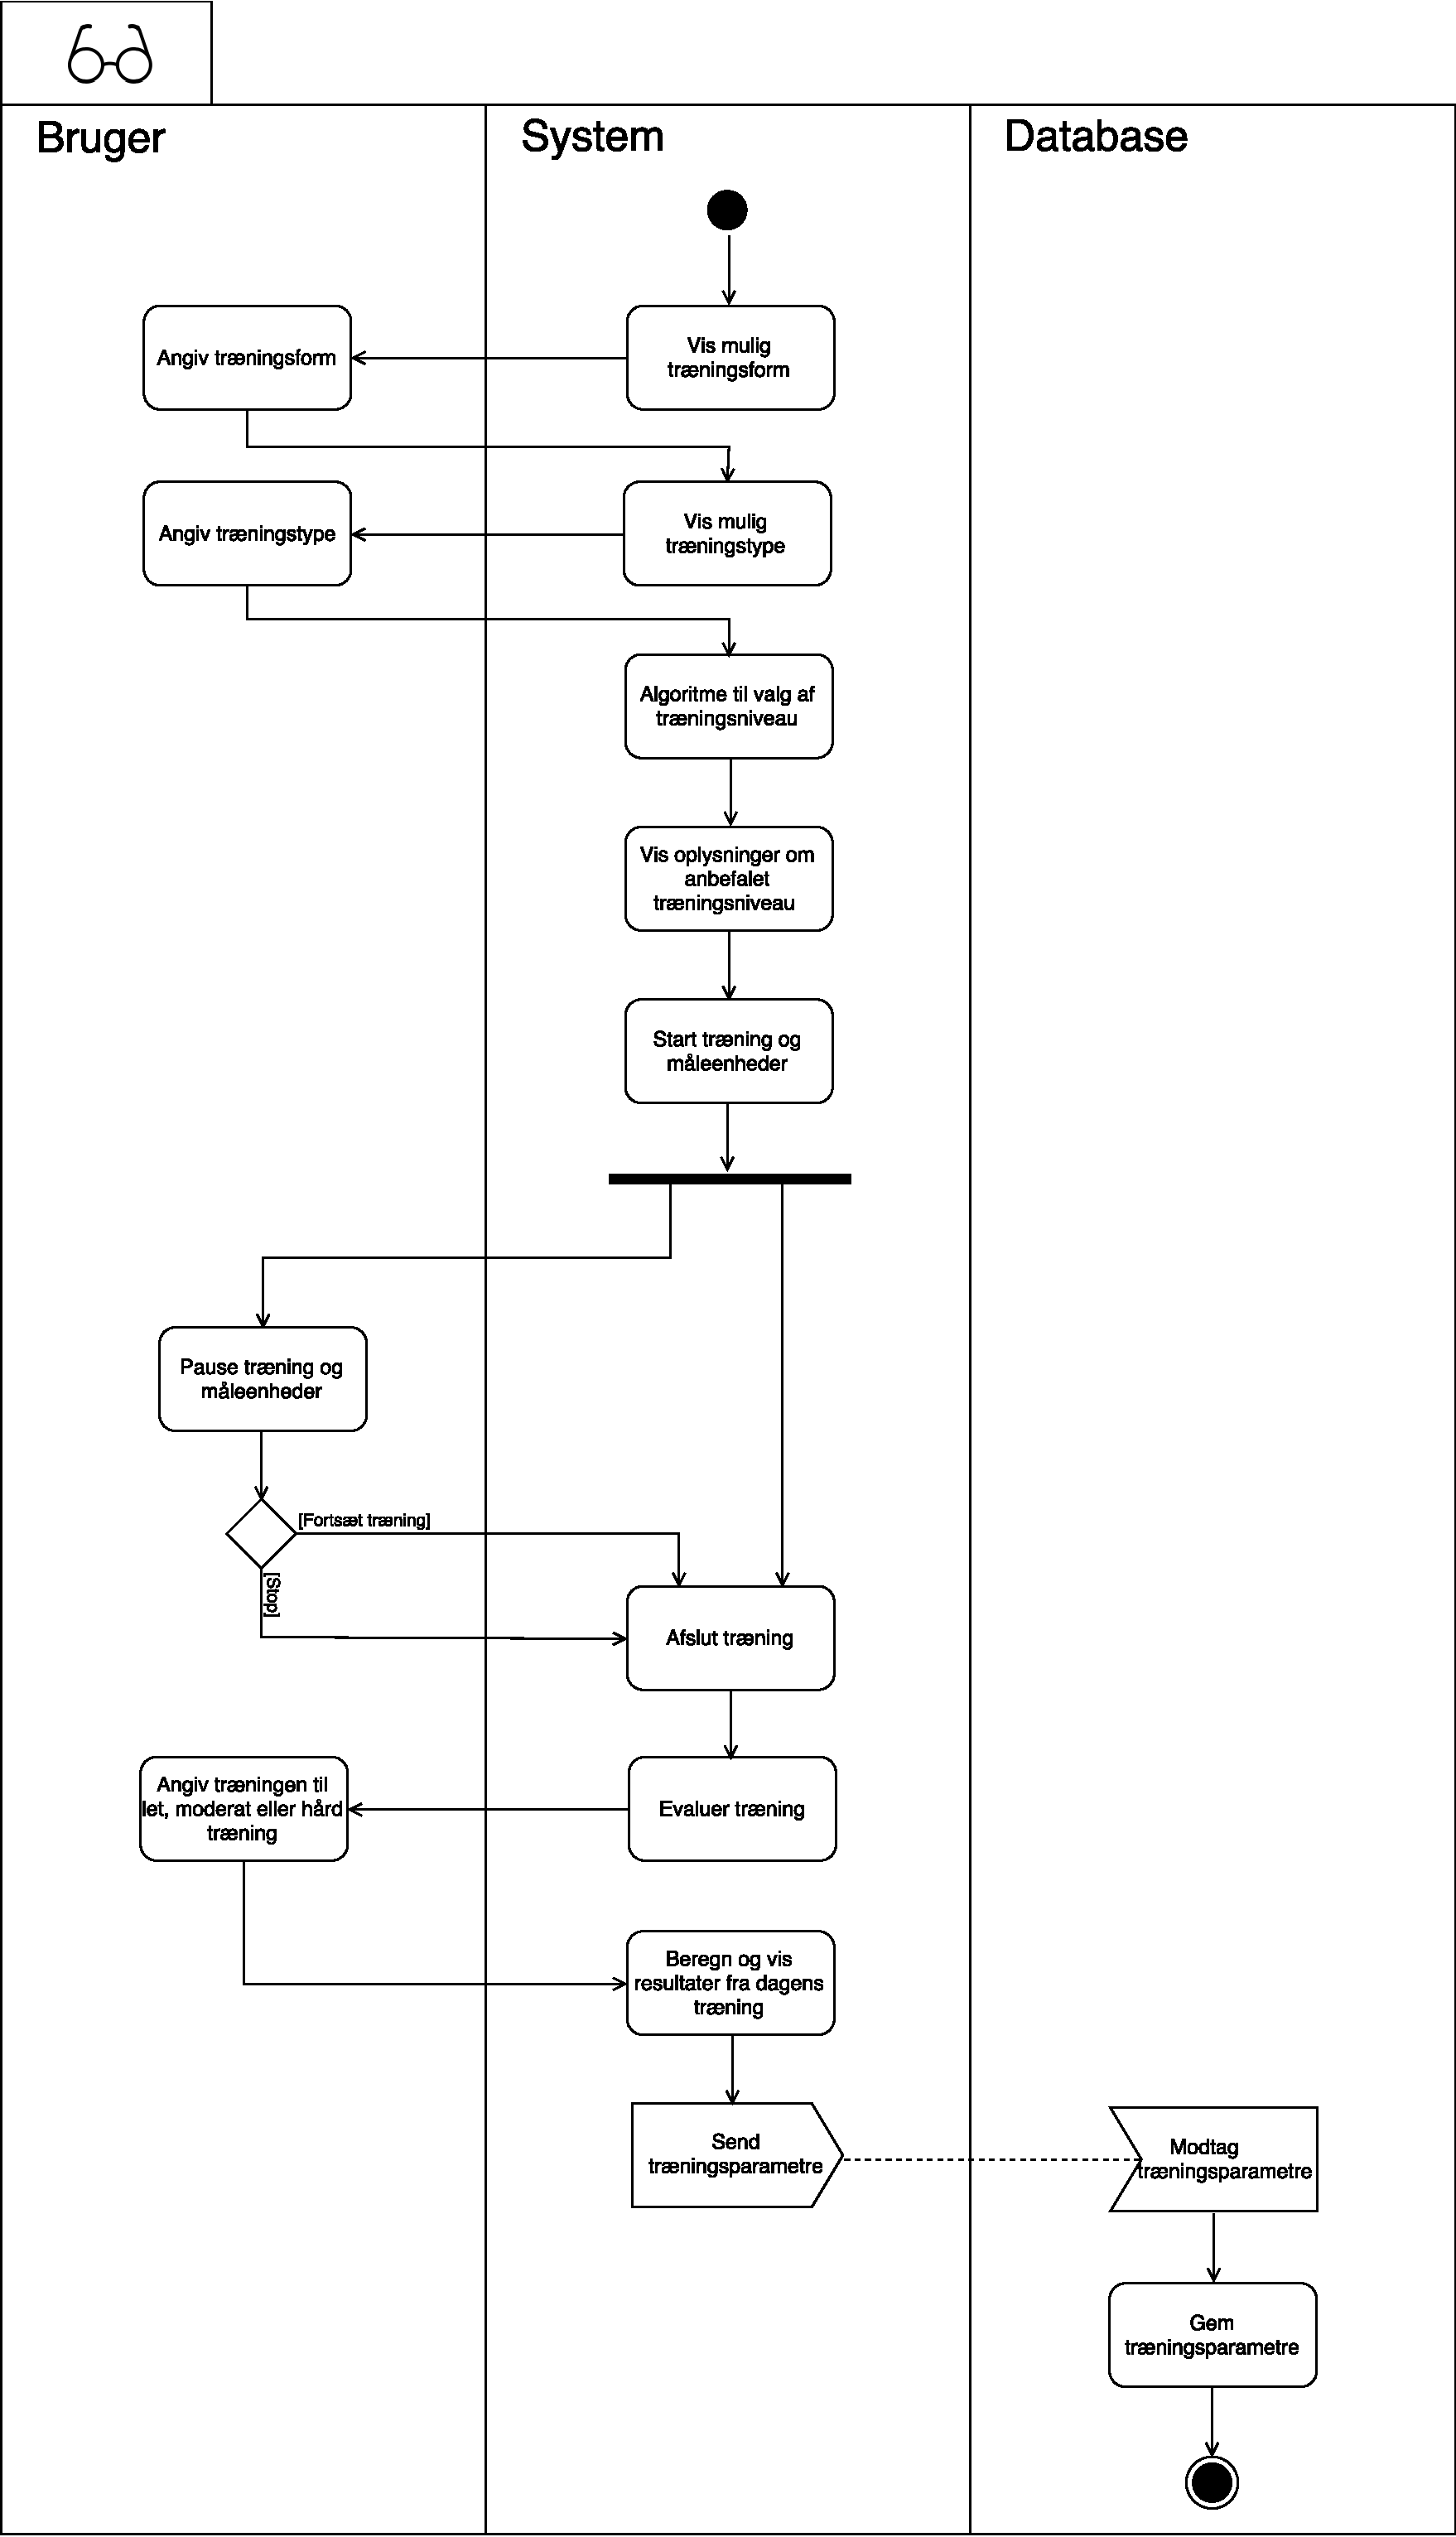
\includegraphics[width=0.8\textwidth]{figures/aktivitetsdiagram/NYTraening}
\caption{Aktivitetsdiagram over træning.}
\label{fig:traening}
\end{figure}

\noindent
Før selve træningen påbegyndes, skal brugeren angive den ønskede træningsform, herunder konditions-, styrketræning eller vejrtrækningsøvelser. Ud fra den valgte træningsform skal brugeren angive træningstype, eksempelvis kan der forekomme gå, løbe eller cykle under konditionstræning. Efterfølgende beregnes et anbefalet træningsniveau ud fra en simpel beslutningstabel, der ses af \autoref{tab:beslutningstabel}. Oplysninger om det anbefalede træningsniveau vises og træningen samt måleenheder kan påbegyndes. 

Under træningen kan brugeren pause træningen, hvorefter det er muligt at fortsætte eller afslutte træningen. Derefter skal brugeren evaluere træningen som værende let, moderat eller hård, hvorefter resultaterne fra den pågældende træning beregnes samt vises. Ligeledes sender systemet træningsparametre, bestående af den daglige helbredstilstand, resultater fra den udførte træning samt evaluering til databasen, som lagrer informationerne. 

\subsubsection*{Algoritme til valg af træningsniveau}
Algoritmen til valg af træningsniveau er illustreret som en simpel beslutningstabel, der viser, hvilke parameter, som ligger til grund for valg af træningsniveau til den enkelte bruger. Af \autoref{tab:beslutningstabel} ses beslutningstabellen for valg af træningsniveau.

\begin{table}[H]
\centering
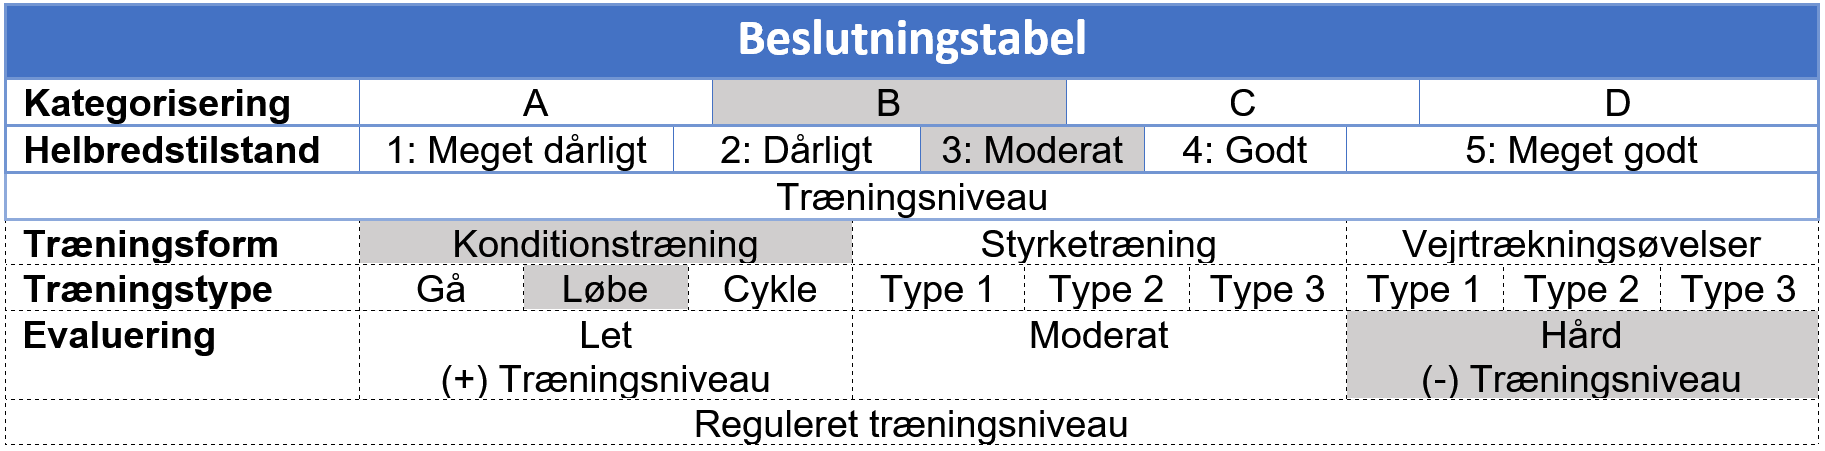
\includegraphics[width=1\textwidth]{figures/aktivitetsdiagram/beslutningstabel}
\caption{Beslutningstabel for træningsniveau. Kategorisering, daglig helbredstilsand samt eventuel evaluering medregnes til at bestemme træningsniveau til den enkelte træning. Af dette eksempel er brugeren kategoriseret B med en helbredstilstand, der er angivet som moderat. Dertil har brugeren valgt løb under konditionstræning. Tidligere har brugeren haft samme daglig helbredstilstand samt træning, og evalueret denne træning som værende hård. Dette muliggøre en regulering af træningsniveauet, hvorfor niveauet i dette tilfælde sænkes.}
\label{tab:beslutningstabel}
\end{table} 

\noindent
Af \autoref{tab:beslutningstabel} fremgår en simpel beslutningstabel for, hvorledes et træningssæt tilpasses den enkelte bruger. Beslutningstabellen tager udgangspunkt i brugerens kategorisering, daglig helbredstilstand samt en eventuel evaluering. Brugeren er i dette tilfælde kategoriseret til B. Helbredstilstanden angives førend en træning påbegyndes, for således at tilpasse niveauet til den pågældende dag. Helbredstilstanden angives efter \textit{1: Meget dårligt}, \textit{2: Dåligt}, \textit{3: Moderat}, \textit{4: Godt} eller \textit{5: Meget godt}, hvortil brugerens helbredstilstand her angives som moderat
Træningsniveauet vurderes dermed ud fra brugerens kategorisering samt helbredstilstand. 
For at have mulighed for at kunne regulere træningssættet yderligere, medregnes den forhenværende evaluering, der er forbundet med samme helbredstilstand, træningsform og type. I dette tilfælde har brugeren før haft samme helbredstilstand, træningsform samt type og dertil evalueret denne træning til værende hård. Algoritmen regulerer hertil træningsniveauet for denne træning ned, for således at give brugeren en bedre træningsoplevelse. 
